\subsection{Caracterización de las palabras identificadas como contrastivas}

\begin{frame}[t]\frametitle{Palabras candidatas}

    \begin{columns}
        \begin{column}{.5\textwidth}
        Para buscar las palabras candidatas a tener contrastes significativos en cuanto a la cantidad de ocurrencias en distintas provincias, elegimos el conjunto de las primeras 
        cinco mil (5000) palabras con mayor valor de nuestra métrica.

        \end{column}

        \begin{column}{.45\textwidth}
            \begin{figure}
            \centering
            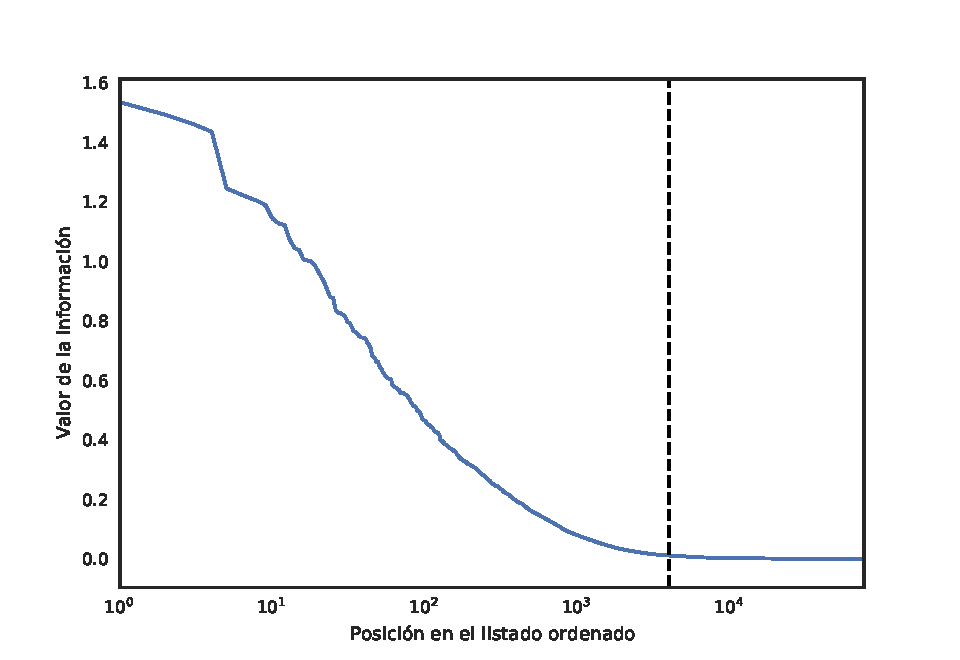
\includegraphics[width=0.95\linewidth]{../src/images2/valorInformacionCorte.pdf}
            \label{fig:ivalue}
            \end{figure}
        \end{column}
    \end{columns}

\end{frame}

\begin{frame}[t]\frametitle{Validación lingüística}

   \begin{itemize}

      \label{it:caracterizacionLinguistica}

      \item \textbf{Coloquialismos o vulgarismos}

      \blockquote[Córdoba]{Perdon pero tenes que ser muy \textbf{culiado/a} para ir a mc y pedirte una ensalada}


      \blockquote[Mendoza]{Q \textbf{chombi} hacer un chiste y q la otra persona no se ría o no lo entienda}

      %   \blockquote[Neuquén]{Que \textbf{carnasas} poniendole rosas rojas a toda la ropa, para mi queda horrible sorry}

      %   \blockquote[Chaco]{Teres, \textbf{pororós} y pelis con Carlita y Flor}

      % \blockquote[San Juan]{Ver un negro \textbf{chuño} con musculosa y gorro.. se ve que el tipo no quería pasar ni frío ni calor.}

      % \blockquote[Formosa]{Tenía la re expectativa para este sábado y al final \textbf{trancó} todo }

      \item \textbf{Indigenismos}

      \blockquote[Formosa]{Te regalo ser \textbf{mitaí} y ir a jurar la bandera con el guardapolvo caliente ese y la corbata que te ahorca todo (Del guaraní mitaí “pequeño”)}

      \blockquote[Corrientes]{\textbf{Angá} mi negrito, esta triste (Del guaraní angá aprox. “pobre”)}

      \item \textbf{Gentilicios}

      \textbf{Casildense} (de Casilda), \textbf{concordiense} (de Concordia) y \textbf{obereño} (de Oberá).

\end{itemize}

% \item \textbf{Voces no marcadas en registro, que aluden a una realidad local}

%   \blockquote[San Juan]{Quiero a alguien que me diga vamos a comer \textbf{piadinas}, un pancho, un chori, una hamburguesa lo que sea y soy feliz}

%   \blockquote[Misiones]{\textbf{Tareferos} que reclamaban asistencia interzafra en Posadas estarían preparando una protesta para hoy en la Fiesta del Inmigrante en Oberá.}

%   \blockquote[Jujuy]{Me encantan los bohemios anti sistema que usan vans. Es como que seas ecologista y uses un cuaderno hecho con media \textbf{yunga}.}

\end{frame}

\begin{frame}[t]\frametitle{Más resultados}
    

\begin{itemize}
  
\item \textbf{Leísmo}

  \blockquote[Misiones]{No te olvides de \textbf{saludarle} a tu suegro hoy}

  \blockquote[Misiones]{Vine a \textbf{visitarle} a mis primas y estan re colgadas, para eso me quedaba en mi casa no maaa }

  \blockquote[Formosa]{A \textbf{esperarle} a nahuel, que traiga los teresss }

% \item \textbf{Fusiones y acrónimos que pueden señalar pronunciación o alta frecuencia de uso}

%   \blockquote[Buenos Aires]{Los sueños de la siesta me dejan \textbf{patra} }

%   \blockquote[Córdoba]{Si mañana me dice q no, voy sola, necesito ver esa pelicula en el cine siosi}

% % \item \textbf{Voces consideradas generales pero que, al aparecer en la lista, permitieron verificar su contrastividad en frecuencia de uso al menos con respecto a España}
%   % Ejemplos: \textbf{pavada}, \textbf{distrital} y \textbf{cariño}.

\item \textbf{Voces sospechadas generales pero con acepción local diferente}

  \blockquote[Mendoza]{Mañana que alguien \textbf{atine} con parque y porrones}

  \blockquote[San Juan]{\textbf{Mansas} ganas de sentarme a tomar un te con semitas}

  \blockquote[Tierra del Fuego]{\textbf{Habilítenme} una nueva espaldaa}

  \blockquote[San Juan]{sigo \textbf{asada} por cosas que han pasado hace como dos dias, que falla (Mendoza) / Que \textbf{asada} estoy, tengo la cabeza echa un lío}


\item \textbf{Voces con una morfología propia de una región}

Ejemplo: terminación azo/aza con base adjetiva.

  \blockquote[San Juan]{Creo que va a estar \textbf{malazo} lo de esta noche } 

  \blockquote[Córdoba]{Esta \textbf{locaza} esa mina para hacer eso}

% \item \textbf{Variantes ortográficas}

%   Ejemplos: culiado (adj. despect. o fórmula de tratamiento de confianza) y tereré.

%   \blockquote[Tucumán]{Menos mal que soy de los chetos de la carne y mañana tengo \textbf{asao} todo el dia jajajajaj}

%   \blockquote[Catamarca]{Un lunes con buen humor ta \textbf{pasao} }

%   \blockquote[Corrientes]{Ahora a la mañana tengo q ir hacerme la tarjebus jajajajj \textbf{mavale} q me estoy por levantarrr jajajaj}  

%   \blockquote[Córdoba]{Q paja volver al colegio \textbf{culiaa}}

%   \blockquote[Córdoba]{Que pajero el \textbf{qliao} este.}

%   \blockquote[Córdoba]{Quiero recitaaal \textbf{qliaaaa}}

%   \blockquote[Entre Ríos]{\textbf{Tereresss} y pile con todos mis primisss}

%   \blockquote[Corrientes]{No se si hacerme un \textbf{tere} o un mate para pasar la siesta}

%   \blockquote[Chaco]{Es lo mas lindo no ir al colegio y quedarme a tomar \textbf{teresss}}


% \item \textbf{Formas verbales coloquiales con sustantivos o adjetivos como base}

%   \blockquote[Neuquén]{Me calma mucho \textbf{mimosear} a mi perro }

%   \blockquote[Buenos Aires]{Me vine a acostar y ya me dicen que parezco de 80 años ME CHUPA UN HUEVO LO QUE PIENSEN, DEJENME \textbf{ABUELEAR} }

%   \blockquote[Tierra del Fuego]{Estaría bueno que ari venga aunque sea a saludarme y que no se quede todo el tiempo \textbf{pollereando}.}


% \item \textbf{Vesres}: Creación de palabras por inversión de sílabas que se usa jergalmente o con fines humorísticos.

%   \blockquote[Corrientes]{Estoy en lo de villa mateando con él y jimmy. Pinta \textbf{sogui} abundante más tarde dijeron }

%   \blockquote[Chaco]{Uhhh me acuerdo si no habré saltado el muro del aguapey par colarme a los \textbf{cequin}. (cequín “fiesta de quince”)}

% \item \textbf{Intejercciones}

%   \blockquote[Formosa]{\textbf{Aijué}, encima me decís vieja, re que no pinta esto facundo jaja ya te dije como es la onda, fin }

%   \blockquote[Formosa]{\textbf{Ains}, una mujer hablando de fútbol.}

%   \blockquote[Corrientes]{Al fin una buena: hora libreeee! \textbf{Yirr} }
% \end{itemize}

\end{itemize}
\end{frame}


\subsection{Validación estadística}

\begin{frame}[t]\frametitle{Problema desde el punto de vista estadístico}


    


\end{frame}

\begin{frame}[t]\frametitle{Test hipergeométrico}

    Para aplicar el test hipergeométrico representamos los datos sobre la palabra en una tabla de 2x2 como la de la siguiente Tabla.

    \begin{table}[ht]
    \centering
    \begin{tabular}{l|ccc}
    \hline
    &  \begin{tabular}{@{}c@{}}\#Palabras \\sobre región\end{tabular} &  \begin{tabular}{@{}c@{}}\#Palabras en el \\ resto de Argentina\end{tabular}  &Total \\ \hline
    \# Palabras w &   $k$ & $K-k$ & $K$ \\ 
    \# Palabras $\neq$ w & $n-k$ & $N + k - n - K$  & $N - K$ \\ \hline
    Total & $n$ & $N -n$ & $N$ \\ 
    \end{tabular}
    \label{tab:contingencia}
    \end{table}

\end{frame}

\begin{frame}[t]\frametitle{Test t de Welch}

    \begin{itemize}
        \item El test de Welch nos provee un valor de probabilidad para rechazar la hipótesis nula que afirma que las medias de las dos distribuciones son iguales.

        \item Las suposiciones del test 
        \begin{enumerate}
            \item Todos los textos son estadísticamente independientes 
            \item La media de las frecuencias proviene de una distribución normal
        \end{enumerate}
        \begin{block}{Metodología}
              Agrupamos todos los tuits de cada usuario representando un texto.\footnote{Notar que la suposición de independencia es más débil.}
        \begin{description}
            \item[Corpus S] Todos los textos de los usuarios que provienen de las provincias en donde se cubre el 80\% de las ocurrencias
            \item[Corpus T] Los textos creados por usuarios del resto de las provincias
        \end{description}

        \end{block}
    \end{itemize}

\end{frame}


\begin{frame}[t]\frametitle{Resultados test t de Welch}

    \begin{columns}[t]
    
        \begin{column}{.3\textwidth}
        La tasa de rechazo de la hipótesis nula en los distintos conjuntos de palabras, los cuales varían según el índice de estas en el listado ordenado según la métrica elegida. 
        \end{column}
        
        \begin{column}{.6\textwidth}
        
            \begin{figure}
            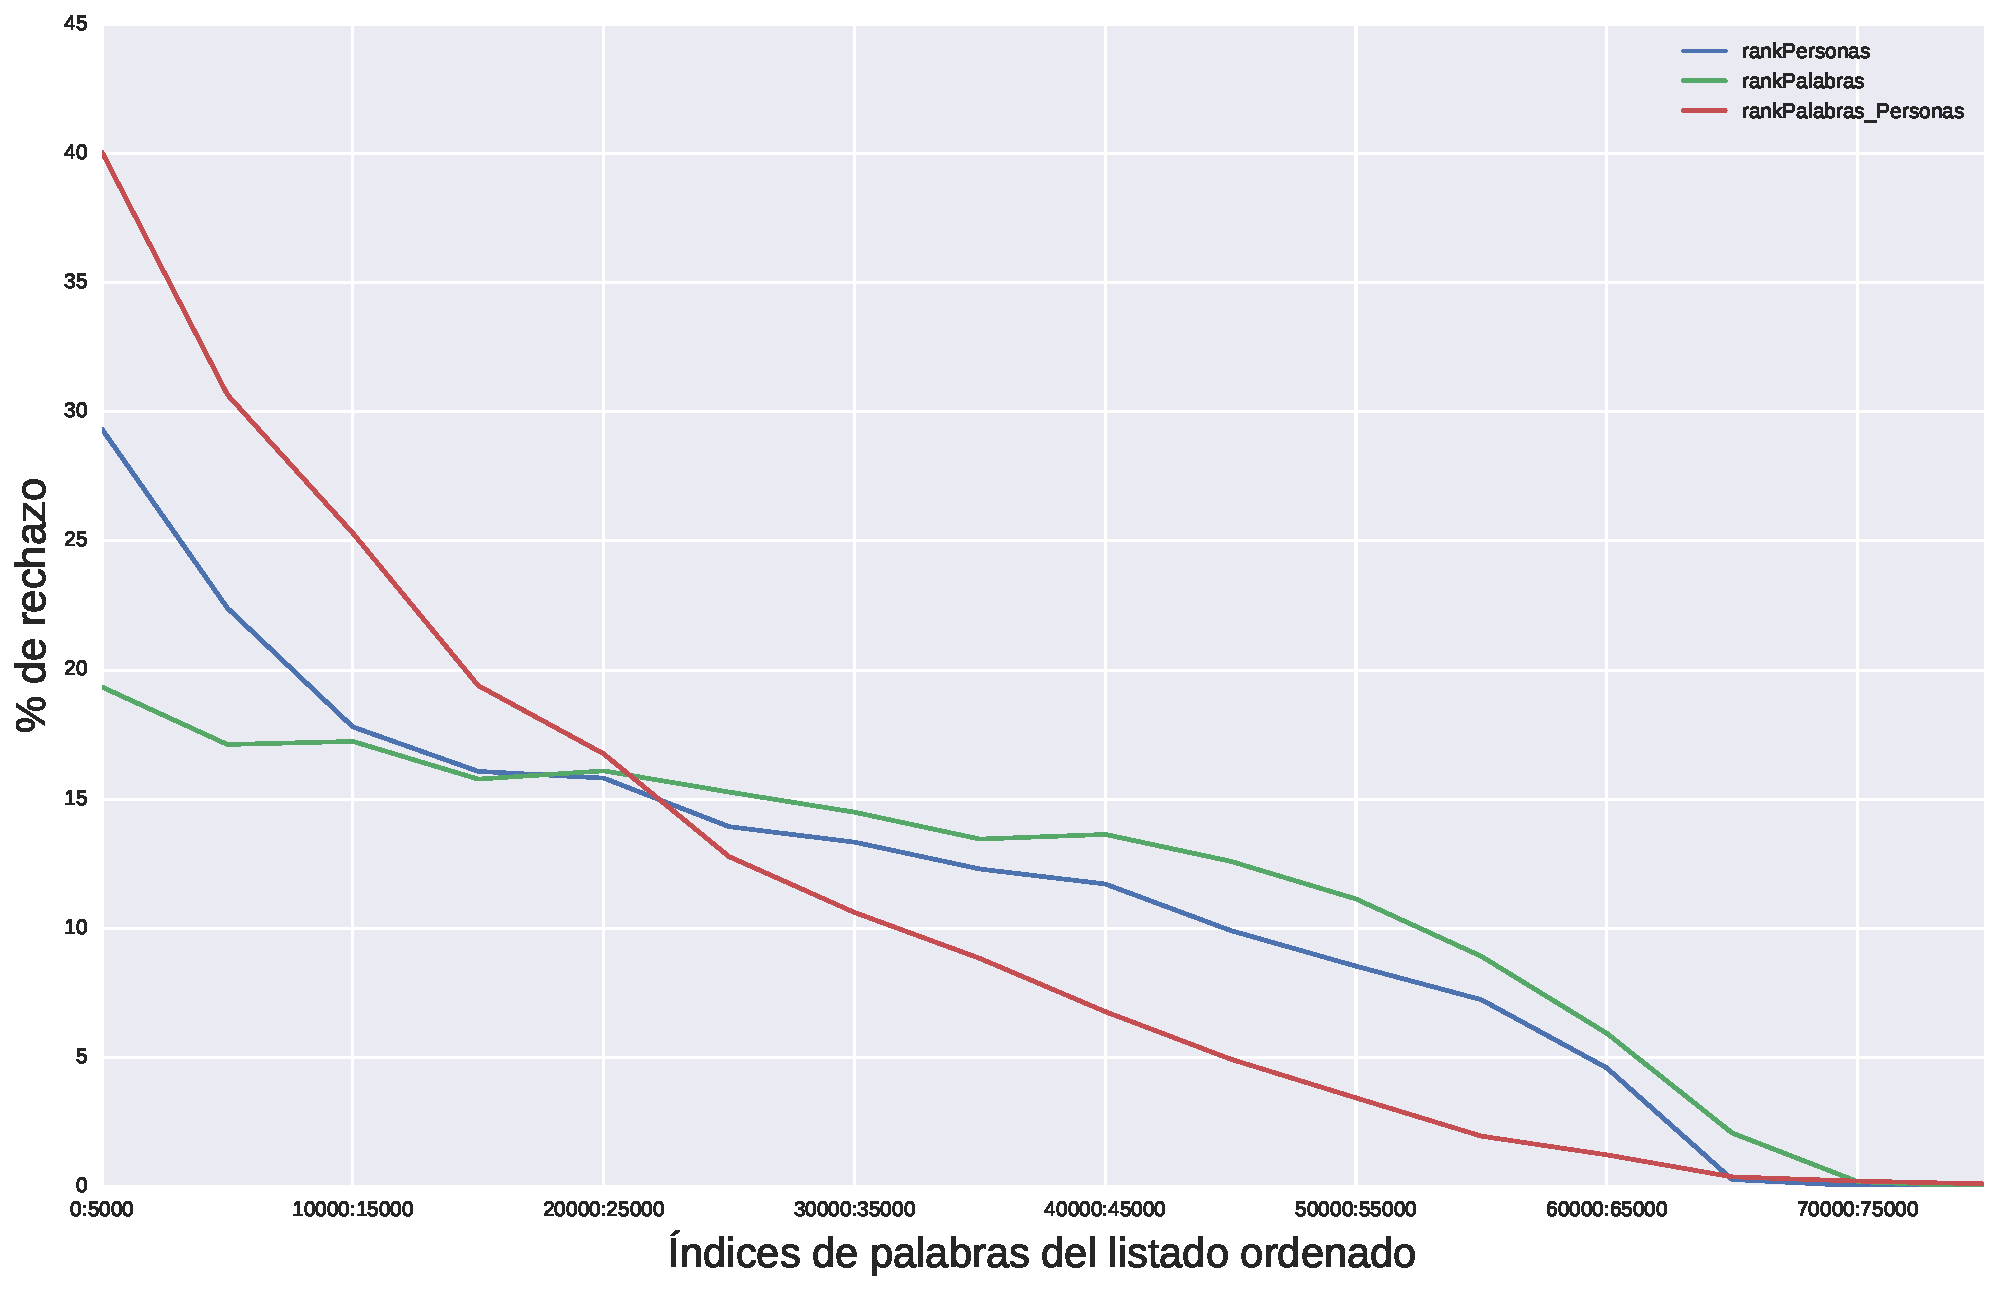
\includegraphics[width=0.95\linewidth]{../src/images/rechazo_metricas.pdf}
            \label{fig:rechazo_metricas}
            \end{figure} 
        \end{column}
    \end{columns}

\end{frame}